Die im Folgenden verwendeten Werte für physikalischen Konstanten werden von \cite{Codata} übernommen.
\subsection{Umrechnung der Messwerte}
Die für jede Frequenz eingestellten Werte an den Drehschrauben sind in Tabelle \ref{tab:Messwerte} zu sehen. Zusätzlich wird der Wert für das vertikale Magnetfeld auf 1.45 eingestellt.
Das Ablesen der Schraubenanzeige ist mit einer Unsicherheit von 0.01 behaftet. Dieser Fehler wird für die Werte der horizontalen und vertikalen Schraube verwendet. Da das Oszilloskop zu Beginn eines Sweep-Intervalls immer einen Ausschlag anzeigt wird die Unsicherheit beim Einstellen der Sweep-Schraube auf die Resonanzstelle auf 0.20 abgeschätzt. \\
Für die Schrauben des horizontalen und des Sweep-Magnetfelds gilt, dass ein Schraubenwert von 10 einem Strom von \SI{1}{\ampere} entspricht. Um auf die Stromstärke zu kommen, werden daher all diese Werte mit 0.1 multipliziert. Bei der Schraube für das vertikale Feld gilt: Ein Schraubenwert von 10 entspricht einem Strom von \SI{3}{\ampere}, d.h. durch die vertikale Spule fließt ein Strom von $1.45\cdot \SI{0.3}{\ampere} = \SI{0.435}{\ampere}$.
\begin{table}
    \centering
    \caption{Stromstärken $I_1,I_2$ beim Auftreten des Maximums für verschiedene Anregungsfrequenzen $\nu_e$ mit dem jeweiligen Skalierungsfaktor}
    \label{tab:Werte}
    \sisetup{parse-numbers=false}
    \begin{tabular}{
	S[table-format=2.3]
	S[table-format=3.0]
	@{${}\pm{}$}
	S[table-format=2.0, table-number-alignment = left]
	S[table-format=3.0]
	@{${}\pm{}$}
	S[table-format=2.0, table-number-alignment = left]
	S[table-format=2.1]
	@{${}\pm{}$}
	S[table-format=1.1, table-number-alignment = left]
	}
	\toprule
	{$\nu_e \ \mathrm{in} \ \si{\mega\hertz}$}		& \multicolumn{2}{c}{$I_1 \ \mathrm{in} \ \si{\milli\ampere}$}		& 
	\multicolumn{2}{c}{$I_2 \ \mathrm{in} \ \si{\milli\ampere}$}		& \multicolumn{2}{c}{Skala in \si{\milli\ampere\per\centi\meter}}		\\ 
	\midrule
    10.588 & 232 & 5  & 307 & 5  & 41.5 & 0.5 \\
15.970 & 357 & 9  & 407 & 5  & 16.7 & 0.3 \\
20.560 & 453 & 9  & 546 & 4  & 18.1 & 0.3 \\
23.870 & 587 & 10 & 633 & 10 & 15.2 & 0.6 \\
29.420 & 717 & 10 & 787 & 8  & 15.3 & 0.4 \\

    \bottomrule
    \end{tabular}
    \end{table}

\clearpage
\subsection{Landé-Faktor und Erdmagnetfeld}
Die Windungsanzahl $N$ und der Radius $R$ aller Spulen sind bekannt, sodass die gemessenen Stromstärken $P$ mit Hilfe von
\begin{align*}
	B = \frac{8\mu_0}{\sqrt{125}}\cdot\frac{P\cdot N}{R}
\end{align*}
in magnetische Feldstärken übersetzt werden können. In horizontaler Richtung wirkt kein Magnetfeld auf das Gas, da das Erdmagnetfeld gerade durch das vertikale Feld einer Helmholtzspule kompensiert wird. Das Gesamtfeld ist demnach die Summe aus Sweep- und Horizontal-Feld. Diese Werte sind für die erste Resonanzstelle $B_1$ und die zweite Resonanzstelle $B_2$ mit der zugehörigen Frequenz in Tabelle \ref{tab:Regression} aufgetragen. An diese Werte wird eine lineare Funktion gefittet, siehe Abbildung \ref{fig:Fit}. Nach \eqref{eq:Resonanz} ist die Steigung $m$ der Geraden
\begin{align*}
	m = \frac{h}{g_F\mu_\text{B}} \ .
\end{align*}
Durch Umstellen ergibt sich so der Landé-Faktor für die beiden Isotope:
\begin{align}\label{eq:LandeExp}
	g_{F1} &= \SI{0.50+-0.01}{}
 \ , \notag \\
	g_{F2} &= \SI{0.35+-0.01}{}
 \ .
\end{align}
Der y-Achsenabschnitt entspricht der horizontalen Komponente des Erdmagnetfelds:
\begin{align}\label{eq:Bhor}
	B_{\text{hor.}1} &= \SI{18+-3}{\micro\tesla}
 \ , \notag \\
	B_{\text{hor.}2} &= \SI{21+-5}{\micro\tesla}
 \ .
\end{align}
Aus der Stromstärke durch die vertikalen Helmholtzspulen kann der Betrag des Magnetfelds in vertikaler Richtung
\begin{align}
	B_\text{vert.} &= \SI{22.2+-0.2}{\micro\tesla}

\end{align}
berechnet werden. Mit diesem Wert und dem Mittelwert aus \eqref{eq:Bhor} wird nun die Stärke des gesamten Erdmagnetfeldes zu
\begin{align}\label{eq:BErdeExp}
	B_\text{Erde} &= \SI{30+-2}{\micro\tesla}

\end{align}
bestimmt.
\begin{figure}
	\centering
	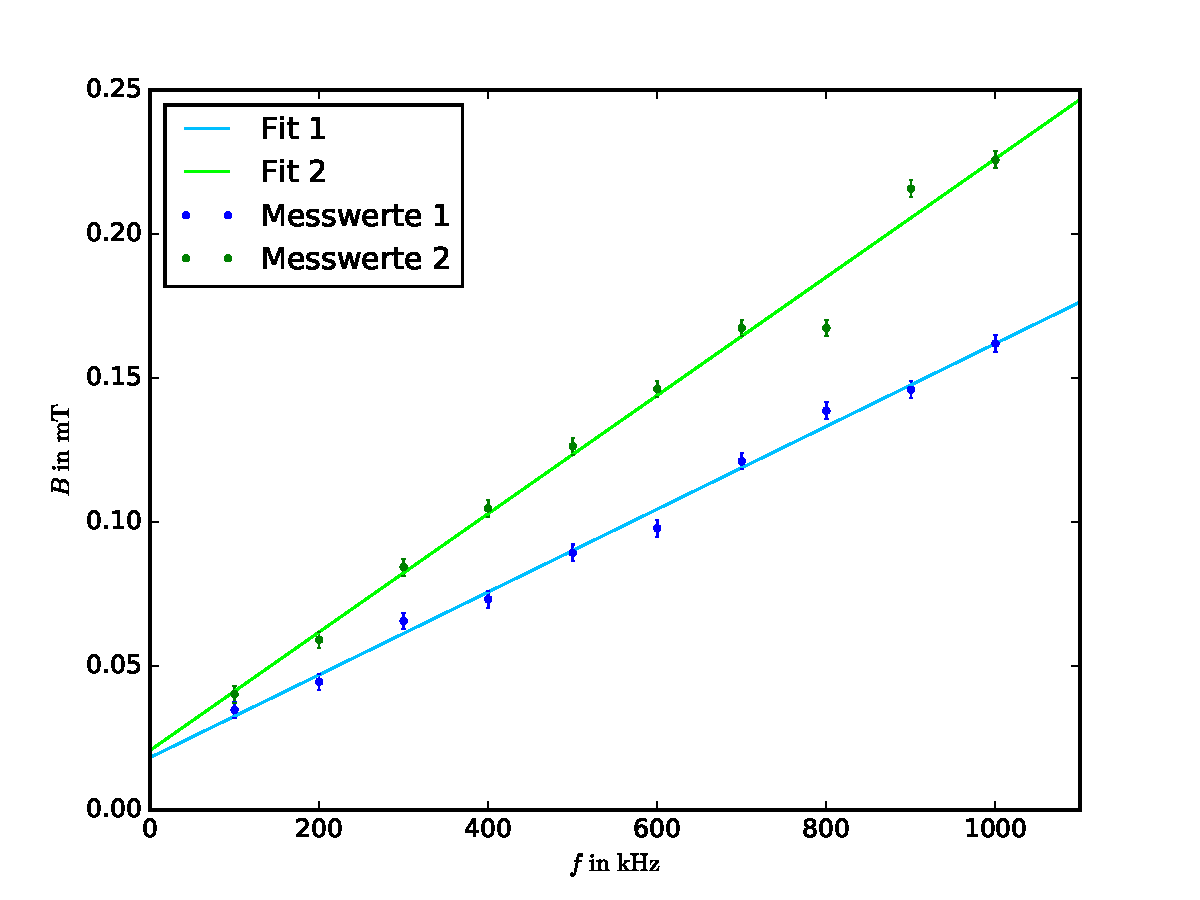
\includegraphics[width=0.7\textwidth]{Fit.pdf}
	\caption{Messwertepaare $\{\nu,B\}$ und Fit für beide Resonanzstellen}
	\label{fig:Fit}
\end{figure}
\begin{table}
    \centering
    \caption{Bei der Regression verwendete Werte}
    \label{tab:Regression}
    \sisetup{parse-numbers=false}
    \begin{tabular}{
	S[table-format=2.3]
	S[table-format=1.2]
	@{${}\pm{}$}
	S[table-format=1.2, table-number-alignment = left]
	}
	\toprule
	{$\nu \ \mathrm{in} \ \si{\mega\hertz}$}		& \multicolumn{2}{c}{$B \ \mathrm{in} \ \si{\milli\tesla}$}		\\ 
	\midrule
    10.588 & 0.378 & 0.005 & 0.052 & 0.005 \\
15.970 & 0.536 & 0.007 & 0.035 & 0.007 \\
20.560 & 0.701 & 0.007 & 0.065 & 0.007 \\
23.870 & 0.86  & 0.01  & 0.03  & 0.01  \\
29.420 & 1.055 & 0.009 & 0.049 & 0.009 \\

    \bottomrule
    \end{tabular}
    \end{table}

\clearpage
\subsection{Kernspin}
Zur Berechnung des Kernspins wird Gleichung \eqref{eq:LandeF} benötigt. Der Gesamtdrehimpuls $F$ wird er durch $J+I$ ersetzt. Es ergibt sich die quadratische Gleichung
\begin{align*}
	I^2 + I\left(J\left(2-\frac{g_J}{g_F}\right)+1\right) + J(J+1)\left(1-\frac{g_J}{g_F}\right) = 0 \ .
\end{align*}
Da Rubidium ein Alkalimetall ($L = 0$) ist, gilt $J=S=\frac{1}{2}$ und $g_J = g_S = 2.00232$. Die (plus-) Lösung für die beiden Isotope ist dann
\begin{align}\label{eq:KernspinExp}
	I_1 &= \SI{1.51+-0.06}{}
 \ , \notag \\
	I_2 &= \SI{2.4+-0.1}{}
 \ .
\end{align}
Die erste Resonanz kommt daher von Rubidium-87 ($I=\frac{3}{2}$) und die zweite von Rubidium-85 ($I=\frac{5}{2}$).
\subsection{Isotopenverhältnis}
Abbildung \ref{fig:Oszilloskop} zeigt das verwendete Bild am Oszilloskop, die verwendeten Größen sind eingezeichnet. Die absoluten und auf 1 normierten Werte, die vom Bild abgelesen werden, sind
\begin{alignat}{3}
	&\text{absolut}	&	&&\text{no}	&	\text{rmiert} \notag \\
	T_\text{max} &= \SI{6.95(50)}{\volt} \qquad& T_\text{max}\ &&= \ &1 \notag \\
	T_0 &= \SI{0}{\volt} 		& T_0\ &&= \ &0 \notag \\
	T_1 &= \SI{5.20(50)}{\volt} & T_1\ &&= \ &\SI{0.108}{\micro\second}
 \notag \\
	T_2 &= \SI{3.60(50)}{\volt} & T_2\ &&= \ &\SI{0.093}{\micro\second}
 \ .
 \end{alignat}
Der Zusammenhang zwischen $T$ und der Anzahl der Besetzung des niedrigsten Niveaus $N_1$ wird als
\begin{align}\label{eq:Transparenz}
	T = 1-\frac{N_1}{N} = 1-\frac{N_{85,1}+N_{87,1}}{N_{85}+N_{87}}
\end{align}
angenommen, wobei $N=N_{85} + N_{87}$ die Gesamtzahl der Atome ist. \\
In der ersten Resonanzstelle sind alle Atome des Isotops Ru-87 im Grundzustand und alle Atome des Isotops Ru-85 angeregt, d.h. $N_{87,1} = N_{87}$,  $N_{85,1}=0$. Eingesetzt in \eqref{eq:Transparenz} gilt daher
\begin{align*}
	T_1 = \frac{N_{85}}{N_{85} + N_{87}} \ .
\end{align*}
Analog kann für die zweite Resonanzstelle der Zusammenhang
\begin{align*}
	T_2 = \frac{N_{87}}{N_{85} + N_{87}}
\end{align*}
aufgestellt werden. Aus dem Quotienten der beiden Transparenzen wird so das Isotopenverhältnis
\begin{align}\label{eq:RatioExp}
	\frac{T_1}{T_2} = \frac{N_{85}}{N_{87}} = \SI{1.5+-0.2}{}

\end{align}
bestimmt.
\begin{figure}
	\centering
	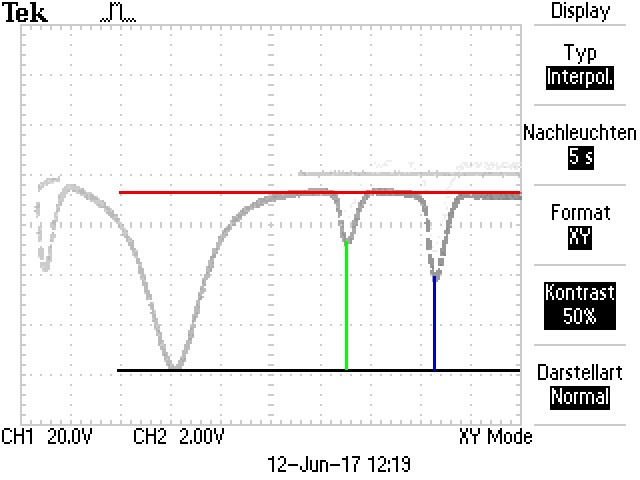
\includegraphics[width=0.5\textwidth]{Oszilloskop/Bearbeitet.JPG}
	\caption[Oszilloskop-Bild]{Oszilloskop-Bild. Die schwarze Linie entspricht $T_0=0$, die rote Linie $T_\text{max}=1$, die grüne Linie $T_1$, die blaue Linie $T_2$.}
	\label{fig:Oszilloskop}
\end{figure}
\subsection{Quadratischer Zeeman-Effekt}
Um den Anteil des quadratischen Zeeman-Effekts zu berechnen wird das Verhältnis $a$ aus dem quadratischen Term und der gesamten Energielücke (Gleichung \eqref{eq:quadrat}) gebildet.
\begin{align}
	a = \frac{g_F^2 \mu_B^2 B^2 \frac{(1-2 M_F)}{\Delta E}}{g_F \mu_B B +g_F^2 \mu_B^2 B^2 \frac{(1-2 M_F)}{\Delta E}}
\end{align}
Da es sich um eine Abschätzung handelt und der Effekt bei zunehmendem Magnetfeld stärker wird, nehmen wir einen Wert für $B$ an, der knapp oberhalb der berechneten Resonanzstellen liegt
\begin{align*}
	B = \si{0.5}{\milli\tesla}
\end{align*}
Die Landé-Faktoren sind in vorherigen Aufgabenteilen bestimmt worden. Als Orientierungszahl $M_F$ wird der Kernspin $I$ eingesetzt. Die Energien $\Delta E$ in in der Anleitung angegeben \cite{\V}.
 Für Rubidium-87 ist das Verhältnis
 \begin{align*}
 	a_1 = \SI{-4.6+-0.1e-27}{}

 \end{align*}
 und für Rubidium-85
  \begin{align*}
  	a_2 = \SI{-6.5+-0.3e-27}{}
 \quad .
  \end{align*}
 